\label{sec:instruction}
\section{Инструкция пользователя}

\begin{enumerate}
    
    \begin{figure}[H]
        \item Запустите программу.
        \vspace{0.3cm}
        

        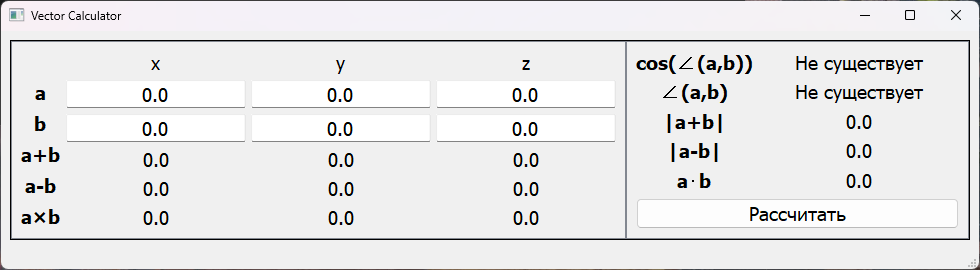
\includegraphics[width=\textwidth]{img//instruction1}
        \caption{}
    \end{figure}

    
    \begin{figure}[H]
        \item Введите желаемые значения координат векторов.
        \vspace{0.3cm}


        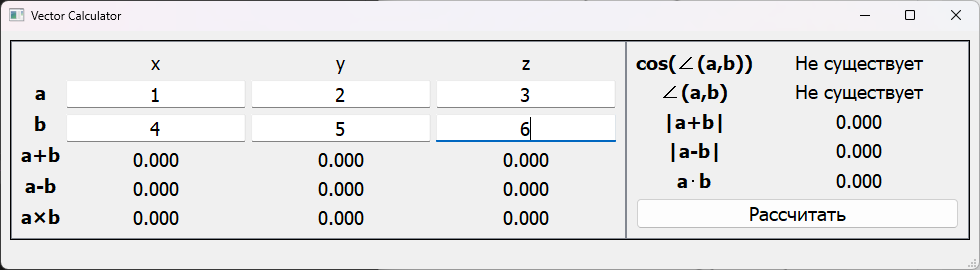
\includegraphics[width=\textwidth]{img//instruction2}
        \caption{}
    \end{figure}


    \begin{figure}[H]
        \item Нажмите кнопку <Рассчитать> и получить значение желаемой величины.
        \vspace{0.3cm}


        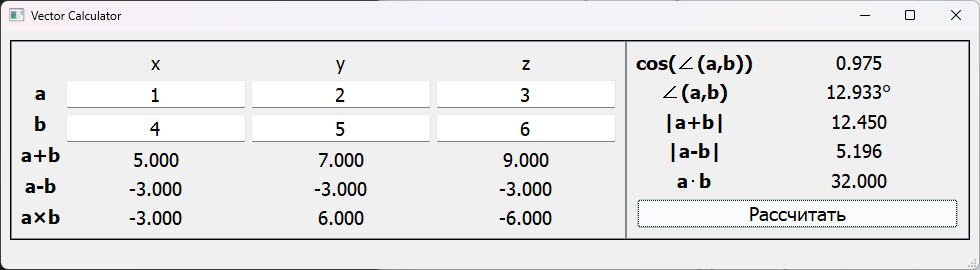
\includegraphics[width=\textwidth]{img//instruction3}
        \caption{}
    \end{figure}

\end{enumerate}